
The system is a layer of fluid between $y=0$ and $y=h$, with boundary conditions $T(x,y=0)=T_b$ 
and $T(x,y=h)=0$, characterized by $\rho_0$, $C_p$, $k$, $\eta_0$ which are assumed to be constant
(in space and time). 


The Stokes equation is $\vec \nabla \cdot \bm \sigma + \rho \vec g = \vec 0$. 
The components of the this equation on the $x$- and $y-$axis are:
\begin{eqnarray}
(\vec \nabla \cdot \bm \sigma)_x &=& - \rho \vec g \cdot \vec e_x = 0 \nn\\ 
(\vec \nabla \cdot \bm \sigma)_y &=& - \rho \vec g \cdot \vec e_y = \rho g_0 \nn
\end{eqnarray}
since $\vec g$ and $\vec e_y$ are in opposite directions ($\vec g = - g_0 \vec e_y$, with $g_0>0$).

Following Eq.~\eqref{eq:md40}, the stream function formulation of the incompressible 
isoviscous Stokes equation is
\[
\eta_0 \nabla^4 \Psi
= \frac{\partial \rho g_y}{\partial x} - \frac{\partial \rho g_x}{\partial y}   
= \frac{\partial \rho g_y}{\partial x} 
= -g_0 \frac{\partial \rho}{\partial x} 
\]
since $g_x=0$ and $g_y=\vec{g}\cdot\vec{e}_y=-g_0$.
Assuming a linearised density field with regards to temperature $\rho(T)=\rho_0 (1-\alpha T)$
we have 
\[
\frac{\partial \rho}{\partial x} 
=
-\rho_0 \alpha \frac{\partial T}{\partial x} 
\]
and then 
\begin{equation}
\vec\nabla^4 \Psi= \frac{\rho_0 g_0 \alpha}{\eta_0} \frac{\partial T}{\partial x} 
\end{equation}
For small perturbations of the conductive state\footnote{The conductive state temperature
is defined as the solution of the steady state diffusion equation $\Delta T_c = 0$ 
subjected to the desired boundary conditions at the top and at the bottom.} $T_c(y)=(1-y/h)T_b$ 
we define the temperature perturbation $\tilde{T}(x,y)$ such that 
\[
T(x,y,t)=T_c(y)+\tilde{T}(x,y,t)
\]
Note that the temperature perturbation $\tilde{T}$ must satisfy the homogeneous boundary 
conditions $\tilde{T}(x,y=0)=0$ and $\tilde{T}(x,y=h)=0$.
We then have\footnote{This is the same equation as in Turcotte \& Schubert, eq 6.310.}: 
\begin{equation}
\boxed{
\vec\nabla^4 \Psi= \frac{\rho_0 g_0 \alpha}{\eta_0} \frac{\partial \tilde{T}}{\partial x} 
}
\label{eq:biharm3}
\end{equation}
In the absence of heat production, the temperature equation (in the Boussinesq approx.) is 
\begin{eqnarray}
 \rho_0 C_p \left( \frac{\partial T}{\partial t} + {\vec \upnu}\cdot {\vec \nabla} T \right) 
= k \Delta T 
\quad
\Rightarrow
\quad
\rho_0 C_p \left( \frac{\partial (T_c+\tilde{T})}{\partial t} + {\vec \upnu}\cdot {\vec \nabla} 
(T_c+\tilde{T}) \right) 
= k \Delta (T_c+\tilde{T})
\end{eqnarray}
First we start by acknowledging that $T_c$ does not depend on time, 
so that $\partial T_c/\partial t = 0$.
Then, $\Delta T_c=0$ since $T_c$ is a linear function of $y$.
Finally, we assume the nonlinear 
term ${\vec \upnu}\cdot {\vec \nabla} \tilde{T} $ to be second order (temperature perturbations and 
coupled velocity changes are assumed to be small).
In the end, defining the heat diffusion coefficient $\kappa$ as $\kappa =k/\rho_0 C_p$, the energy equation can be simplified further as follows:
\[
%\rho_0 C_p \left( \frac{\partial \tilde{T}}{\partial t} + {\vec \upnu}\cdot {\vec \nabla} T_c \right) 
%= k \Delta \tilde{T}
%\qquad
%\Rightarrow
%\qquad
\frac{\partial \tilde{T}}{\partial t} + {\vec \upnu}\cdot {\vec \nabla} T_c 
= \kappa \Delta \tilde{T}
\]
Using the relationship between velocity and stream function
$\vec\upnu=(u,v)=(\partial_y \Psi, -\partial_x \Psi)$ and 
since $\vec\nabla T_c = - (T_b/h) \vec{e}_y$ then
\[
{\vec \upnu}\cdot {\vec \nabla} T_c =
\left(
\begin{array}{c}
\partial_y \Psi \\ 
-\partial_x \Psi
\end{array}
\right)
\cdot
\left(
\begin{array}{c}
0 \\ 
- T_b/h
\end{array}
\right)
=
\frac{T_b}{h}   \frac{\partial \Psi}{\partial x} 
\]
and finally\footnote{This is the same equation as in Turcotte \& Schubert, eq 6.309.}:
\begin{equation}
\boxed{
\frac{\partial \tilde{T}}{\partial t} - \kappa \Delta \tilde{T} 
= -  \frac{T_b}{h}   \frac{\partial \Psi}{\partial x}
}
\label{eq:biharm1}
\end{equation}
%We also have [{\color{red} prove}]
%\[
%{\bm \nabla}^4 \Psi = -Ra \frac{\partial T_1}{\partial %x}
%\]


Looking at these equations, we immediately think about a separation of variables approach to solve these equations. Both equations showcase the Laplace operator $\Delta$, and the eigenfunctions of the biharmonic operator and the Laplace operator are the same. 
We then pose that $\Psi$ and $\tilde{T}$ can be written\footnote{T \& S actually very much postulate the final form of these quantities without (enough?) justification. I would like to revisit this in the future and better support this assertion.
}:
\[
\tilde{T}(x,y,t) = \tilde{T}_0 \exp(pt) 
\left[a_k \cos(k_x x) + b_k \sin(k_x x) \right]
\left[c_k \cos(k_y y) + d_k \sin(k_y y) \right]
\]
\[
\Psi(x,y,t)=
\Psi_0 \exp(pt) 
\left[\alpha_k \cos(k_x x) + \beta_k \sin(k_x x) \right]
\left[\delta_k \cos(k_y y) + \gamma_k \sin(k_y y) \right] 
\]
where $\tilde{T}_0$ and $\Psi_0$, $a_k,b_k,c_k,d_k$ and $\alpha_k,\beta_b,\delta_k,\gamma_k$ are constants.
We then of course have 
\begin{eqnarray}
\vec\nabla^2 \tilde{T} 
&=& \frac{\partial^2 \tilde{T}}{\partial x^2 } + \frac{\partial^2 \tilde{T}}{\partial y^2 }  \nn\\
&=& \tilde{T}_0 \exp (pt) 
\left\{
\left[-k_x^2 a_k \cos(k_x x) -k_x^2 b_k \sin(k_x x) \right]
\left[c_k \cos(k_y y) + d_k \sin(k_y y) \right]
\right\} \nn\\
&+& \tilde{T}_0 \exp (pt) 
\left\{
\left[a_k \cos(k_x x) + b_k \sin(k_x x) \right]
\left[-k_y^2 c_k \cos(k_y y) -k_y^2 d_k \sin(k_y y) \right]
\right\} \nn\\
&=& -(k_x^2 + k_y^2) \tilde{T} \label{eigenTtilde}
\end{eqnarray}
and a similar expression for $\Psi$.

The boundary conditions on $\tilde{T}$ are $\tilde{T}(y=0)=\tilde{T}(y=h)=0$.
From the first one it follows immediately that $c_k=0$. 
From the second, we arrive at $k_y h = n \pi$, which yields $\sin ( n \pi y/h)$
where $n$ is an integer.
We then arrive at the following expression for the temperature $\tilde{T}$:
\[
\tilde{T}(x,y,t) = 
\tilde{T}_0 \exp(pt) 
\left[a_k \cos(k_x x) + b_k \sin(k_x x) \right]
\sin \left(n\pi \frac{y}{h} \right)
\]
where $n$ is an integer number.

At this stage we make an important assumption:
at $t=0$ we then only consider a single horizontal periodic perturbance 
with wavelength $\lambda$ as depicted below. In such a case we expect that 
it would in fact lead to the formation of the following convection cells:

\begin{center}
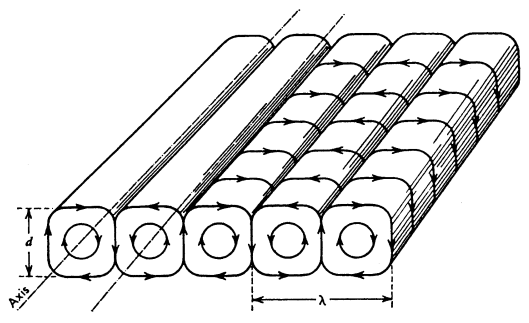
\includegraphics[width=8cm]{images/chapter_md/RBcells}\\
{\captionfont Note that the number of cells left and right of those shown is infinite.
Source unknown. The coordinate $x=0$ is set to the left vertical dashed line 
for convenience.}
\end{center}

The boundary conditions are free slip at the top and at the bottom, i.e.
$v(y=0)=v(y=h)=0$.
Also, by symmetry of the perturbance we see that $u=0$ at each 'side' (i.e.
on the vertical dashed lines of the figure above), 
i.e. for $x=0$ and $x=\lambda$.

Let us now turn to the vertical $y$ component of the velocity:
\begin{eqnarray}
v 
&=& -\frac{\partial \Psi}{\partial x}  \nn\\
&=& -\frac{\partial }{\partial x} 
\left\{
\Psi_0 \exp(pt) 
\left[\alpha_k \cos(k_x x) + \beta_k \sin(k_x x) \right]
\left[\delta_k \cos(k_y y) + \gamma_k \sin(k_y y) \right] 
\right\}
\nn\\
&=& - \Psi_0 \exp(pt) 
\left[- \alpha_k k_x \sin(k_x x) + \beta_k k_x \cos(k_x x) \right]
\left[\delta_k \cos(k_y y) + \gamma_k \sin(k_y y) \right] 
\end{eqnarray}
The boundary condition at the bottom is $v(y=0)=0$, so that $\delta_k=0$ here again.
The boundary condition at the top is $v(y=h)=0$, so that $k_y h = n \pi=0$ as before.
Then 
\[
\Psi(x,y,t) = 
\Psi_0 \exp(pt) 
\left[\alpha_k \cos(k_x x) + \beta_k \sin(k_x x) \right]
\sin \left( n \pi \frac{y}{h} \right)
\]
Turning now to the horizontal component of the velocity:
\begin{eqnarray}
u 
&=& \frac{\partial \Psi}{\partial y}  \nn\\
&=& \frac{\partial }{\partial y}  
\left\{
\Psi_0 \exp(pt) 
\left[\alpha_k \cos(k_x x) + \beta_k \sin(k_x x) \right]
\sin \left( n \pi \frac{y}{h} \right)
\right\}
\nn\\
&=&
\Psi_0 \exp(pt) 
\left[\alpha_k \cos(k_x x) + \beta_k \sin(k_x x) \right]
\frac{n \pi}{h}\sin \left( n \pi \frac{y}{h} \right)
\end{eqnarray}

Using now the 'side' boundary conditions:
$u(x=0)=0$ yields $\alpha_k=0$ and $u(x=\lambda)=0$ yields $k_y \lambda = 2\pi$
so that in the end:
\begin{equation}
\boxed{
\Psi(x,y,t) = 
\Psi_0 \exp(pt) 
\sin \left(\frac{2\pi}{\lambda} x \right) 
\sin \left(\frac{n \pi }{h}y \right)
}
\label{eq:psi2}
\end{equation}





Looking at the biharmonic equation \eqref{eq:biharm1}, its rhs is $\sim \frac{\partial \Psi}{\partial x}$.
Then, the $x$ dependency of this term will be $\cos(2 \pi x / \lambda)$.
The lhs term of \eqref{eq:biharm1} is proportional to $\tilde{T}$ (see Eq.~\eqref{eigenTtilde}), i.e. proportional to $ a_k \cos (k_x x) + b_k \sin (k_x x)$.
For these equations to be compatible, we must set $b_k=0$ and we then obtain\footnote{
Taking $n=1$ and remembering that Turcotte \& Schubert have the domain between 
$y-h/2$ and $y=h/2$, these expressions are identical to Eqs. 6.311 and 6.312 
of the book. Also one could have assigned $\partial T/\partial x$ on the sides
for symmetry reasons and have obtained the same expression.
}

\begin{equation}
\boxed{
\tilde{T}(x,y,t) = 
\tilde{T}_0 \exp(pt) 
\cos \left( \frac{2\pi}{\lambda} x \right) 
\sin \left(n\pi \frac{y}{h} \right)
}
\label{eq:Ttilde2}
\end{equation}
where $a_k$ has been 'absorbed' in $\tilde{T}_0$.








Then the two framed PDEs above, Eq.~\eqref{eq:biharm3} and Eq.~\eqref{eq:biharm1},
when coupled with Eq.~\eqref{eq:psi2} and  Eq.~\eqref{eq:Ttilde2}, become:
\begin{eqnarray}
%&& \nabla^4 \Psi= -\frac{\rho_0 g_0 \alpha}{\eta_0} \frac{\partial T}{\partial x} \nn \\
%&\Rightarrow& \nabla^4 \Psi= -\frac{\rho_0 g_0 \alpha}{\eta_0} 
%\frac{\partial (T_c(y)+\tilde{T}(x,y))}{\partial x} \nn \\
&& \nabla^4 \Psi= \frac{\rho_0 g_0 \alpha}{\eta_0} \frac{\partial \tilde{T}}{\partial x} \nn \\
&\Rightarrow& \nabla^2  \left[\left( -\frac{4\pi^2}{\lambda^2} - \frac{n^2\pi^2}{h^2} \right) \Psi \right] 
= \frac{\rho_0 g_0 \alpha}{\eta_0} \frac{\partial \tilde{T}}{\partial x} \nn\\
&\Rightarrow& \left( -\frac{4\pi^2}{\lambda^2} - \frac{n^2\pi^2}{h^2} \right)^2 \Psi 
= \frac{\rho_0 g_0 \alpha}{\eta_0} \frac{\partial \tilde{T}}{\partial x} 
\nn\\
&\Rightarrow& \left( \frac{4\pi^2}{\lambda^2} + \frac{n^2\pi^2}{h^2} \right)^2
\Psi_0 \exp(pt) 
\sin \left(\frac{2\pi}{\lambda} x \right) 
\sin \left(n\pi \frac{y}{h} \right)
=
\frac{\rho_0 g_0 \alpha}{\eta_0} \cdot - \frac{2 \pi }{\lambda}
\tilde{T}_0 \exp(pt) 
\sin \left( \frac{2\pi}{\lambda} x \right) 
\sin \left(n\pi \frac{y}{h} \right) 
\nn\\
&\Rightarrow& 
\left( \frac{4\pi^2}{\lambda^2} + \frac{n^2\pi^2}{h^2} \right)^2
\Psi_0 
=
-\frac{\rho_0 g_0 \alpha}{\eta_0}  \frac{2 \pi }{\lambda}
\tilde{T}_0 
\\
\nn\\
&& \frac{\partial \tilde{T}}{\partial t} - \kappa \Delta \tilde{T} 
= -  \frac{T_b}{h}   \frac{\partial \Psi}{\partial x} \nn\\
&\Rightarrow & p \tilde{T} - \kappa \left(-\frac{4\pi^2}{\lambda^2} - \frac{n^2\pi^2}{h^2}\right) \tilde{T}   
= -  \frac{T_b}{h}   \cdot  \frac{2 \pi}{\lambda} \Psi_0 \exp(pt)  
\cos \left(\frac{2\pi}{\lambda} x \right) 
\sin \left(n\pi \frac{y}{h} \right) \nn\\
&\Rightarrow & 
\left[ p  + \kappa \left(\frac{4\pi^2}{\lambda^2} + \frac{n^2\pi^2}{h^2}\right) \right]
\tilde{T}_0 \exp(pt) 
\cos \left( \frac{2\pi}{\lambda} x \right) 
\sin \left(n\pi \frac{y}{h} \right)
= -  \frac{T_b}{h}   \frac{2 \pi}{\lambda} \Psi_0 \exp(pt)  
\cos \left(\frac{2\pi}{\lambda} x \right) 
\sin \left(n\pi \frac{y}{h} \right) \nn\\
&\Rightarrow & 
\left[ p  + \kappa \left(\frac{4\pi^2}{\lambda^2} + \frac{n^2\pi^2}{h^2}\right) \right]
\tilde{T}_0 
= -  \frac{T_b}{h}   \frac{2 \pi}{\lambda} \Psi_0 
\end{eqnarray}
We are then left with two equations:
\begin{eqnarray}
\left[ p  + \kappa \left(\frac{4\pi^2}{\lambda^2} + \frac{n^2\pi^2}{h^2}\right) \right]\tilde{T}_0 
&=& -  \frac{T_b}{h}   \frac{2 \pi}{\lambda} \Psi_0 \nn\\
\left( \frac{4\pi^2}{\lambda^2} + \frac{n^2\pi^2}{h^2} \right)^2 \Psi_0 
&=& -\frac{\rho_0 g_0 \alpha}{\eta_0}  \frac{2 \pi }{\lambda} \tilde{T}_0  \nn
\end{eqnarray}
which we can cast as
\[
\left(
\begin{array}{cc}
p  + \kappa \left(\frac{4\pi^2}{\lambda^2} + \frac{n^2\pi^2}{h^2}\right) 
& 
\frac{T_b}{h}   \frac{2 \pi}{\lambda} 
\\
-\frac{\rho_0 g_0 \alpha}{\eta_0}  \frac{2 \pi }{\lambda}
&
-\left( \frac{4\pi^2}{\lambda^2} + \frac{n^2\pi^2}{h^2} \right)^2
\end{array}
\right)
\left(
\begin{array}{c}
\tilde{T}_0 \\ \\ \Psi_0
\end{array}
\right)
=
\left(
\begin{array}{c}
0 \\ \\ 0
\end{array}
\right)
\]
The determinant of the matrix should be zero to have non-trivial solutions\footnote{
Let us consider the following matrix
\[
\left(\begin{array}{cc}
a & b \\ c & d
\end{array}\right)
\cdot
\left(\begin{array}{cc}
x \\ y
\end{array}\right)
=
\left(\begin{array}{cc}
0 \\ 0
\end{array}\right)
\qquad
\Rightarrow
\qquad
\left(\begin{array}{cc}
ac & bc \\ 0 & ad-bc
\end{array}\right)
\cdot
\left(\begin{array}{cc}
x \\ y
\end{array}\right)
=
\left(\begin{array}{cc}
0 \\ 0
\end{array}\right)
\]
where we have multiplied the first row by $c$ and the second row by $a$ and subtract row 1 from row 2. The lower right term $ad-bc$ is the determinant and we find that it must be equal to zero
since $y$ is not zero.
}
for the amplitude factors (i.e. $\tilde{T}_0=0$ and $\Psi_0=0$ which is not helpful).
This leads to the condition: 
\begin{eqnarray}
Det &=& 
\left[ p  + \kappa \left(\frac{4\pi^2}{\lambda^2} + \frac{n^2\pi^2}{h^2}\right)  \right]
\cdot 
-\left( \frac{4\pi^2}{\lambda^2} + \frac{n^2\pi^2}{h^2} \right)^2
+
\frac{\rho_0 g_0 \alpha}{\eta_0}  \frac{2 \pi }{\lambda} 
\cdot
\frac{T_b}{h}   \frac{2 \pi}{\lambda}  \nn\\
&=& -\left[ p  + \kappa \left(\frac{4\pi^2}{\lambda^2} + \frac{n^2\pi^2}{h^2}\right)  \right]
\left( \frac{4\pi^2}{\lambda^2} + \frac{n^2\pi^2}{h^2} \right)^2
+
\frac{\rho_0 g_0 \alpha T_b}{ h\eta_0}  \frac{4 \pi^2 }{\lambda^2}      \nn\\
&=&
- p  \left( \frac{4\pi^2}{\lambda^2} + \frac{n^2\pi^2}{h^2} \right)^2
- \kappa \left(\frac{4\pi^2}{\lambda^2} + \frac{n^2\pi^2}{h^2}\right)^3  
+ \frac{\rho_0 g_0 \alpha T_b}{ h\eta_0}  \frac{4 \pi^2 }{\lambda^2}     \nn
\end{eqnarray}
The determinant is zero for  
\begin{eqnarray}
p  \left( \frac{4\pi^2}{\lambda^2} + \frac{n^2\pi^2}{h^2} \right)^2
&=&
- \kappa \left(\frac{4\pi^2}{\lambda^2} + \frac{n^2\pi^2}{h^2}\right)^3  
+ \frac{\rho_0 g_0 \alpha T_b}{ h\eta_0}  \frac{4 \pi^2 }{\lambda^2}     \nn\\
p 
&=& \frac{
-\kappa \left(\frac{4\pi^2}{\lambda^2} + \frac{n^2\pi^2}{h^2}\right)^3  
+ \frac{\rho_0 g_0 \alpha T_b}{ h\eta_0}  \frac{4 \pi^2 }{\lambda^2}  }
{\left( \frac{4\pi^2}{\lambda^2} + \frac{n^2\pi^2}{h^2} \right)^2} \nn\\
&=& \kappa \frac{
-\left(\frac{4\pi^2}{\lambda^2} + \frac{n^2\pi^2}{h^2}\right)^3  
+ \frac{\rho_0 g_0 \alpha T_b}{ h \kappa \eta_0}  \frac{4 \pi^2 }{\lambda^2}  }
{\left( \frac{4\pi^2}{\lambda^2} + \frac{n^2\pi^2}{h^2} \right)^2} \nn\\
&=& \frac{ \kappa }{h^6}\frac{ -h^6
\left(  \frac{4\pi^2}{\lambda^2} + \frac{n^2\pi^2}{h^2}\right)^3  
+ \frac{\rho_0 g_0 \alpha T_b h^3}{  \kappa \eta_0}  \frac{4 \pi^2 h^2}{\lambda^2}  }
{  \left( \frac{4\pi^2}{\lambda^2} + \frac{n^2\pi^2}{h^2} \right)^2} \nn\\
&=& \frac{ \kappa }{h^2} \frac{- h^6 \left( \frac{4\pi^2}{\lambda^2} + \frac{n^2\pi^2}{h^2}\right)^3  
+ \Ranb \frac{4 \pi^2 h^2}{\lambda^2}  }
{ h^4  \left( \frac{4\pi^2}{\lambda^2} + \frac{n^2\pi^2}{h^2} \right)^2} \nn\\
&=& \frac{ \kappa }{h^2} \frac{ 
-\left( \frac{4\pi^2 h^2}{\lambda^2} + n^2\pi^2 \right)^3  
+ \Ranb \frac{4 \pi^2 h^2}{\lambda^2}  }
{   \left( \frac{4\pi^2 h^2}{\lambda^2} + n^2\pi^2 \right)^2} 
\end{eqnarray}

where we have used the Rayleigh number of the system defined as 
\[
\Ranb= \frac{\rho_0 g_0 \alpha T_b h^3}{\eta_0 \kappa}
\]


The coefficient $p$ inside $\exp(pt)$ present in both temperature and stream function expressions determines the stability of the system: if it is negative, 
the system is stable and both $\Psi$ and $\tilde{T}$ will decay to zero (return to conductive state). 
If $p=0$, then the system is meta-stable, and if $p>0$ then the system is unstable and 
the perturbations will grow. 

In case of the stable regime an initial temperature perturbation will die out (e.g. because conduction wins from advection). In the case of the unstable regime convection will occur with an exponential growth factor. The intermediate, marginally stable, regime is the transition between convection and no convection for which our linearization applies.

The threshold is then $p=0$ and the corresponding critical Rayleigh number $\Ranb_c$ 
is\footnote{this is eq 6.319 of T\&S for n=1}:
\[
\Ranb_c= \frac{ \left( \frac{4\pi^2 h^2}{\lambda^2} + n^2\pi^2 \right)^3   }
{\frac{4 \pi^2 h^2}{\lambda^2}}
\]
Let us denote $\underline{h}=2 \pi h/\lambda$ the dimensionless thickness of the layer.
The critical Rayleigh number is then a function of $\underline{h}$:
\[
\Ranb_c(\underline{h}) = \frac{(\underline{h}^2 + n^2 \pi^2)^3}{\underline{h}^2}
\]
It is plotted on the following figure for $n=1$:

\begin{center}
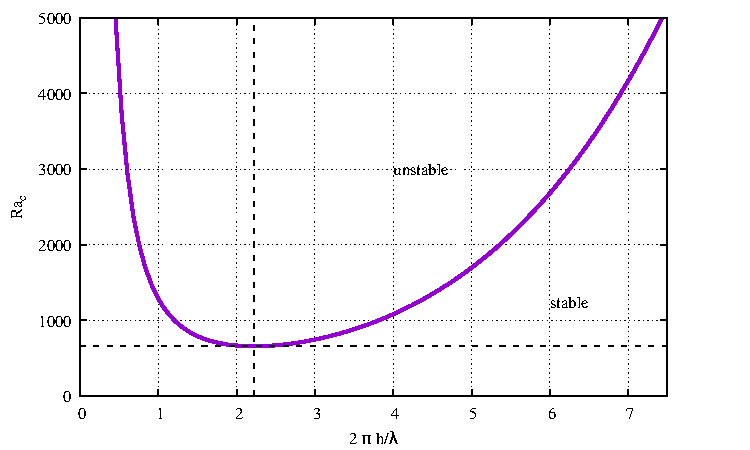
\includegraphics[width=11cm]{images/chapter_md/Ra}\\
{\captionfont 
Critical Rayleigh number $\Ranb_c$ for the onset of
convection in a layer heated from below with stress-free
boundaries as a function of dimensionless wavenumber $2 \pi h/\lambda$ and for $n=1$.
For a system with $\Ranb=2000$ then convection cannot occur for $2 \pi h/\lambda< 0.8$ and 
$2 \pi h/\lambda > 5.4$. The dashed lines indicate the minimum critical Rayleigh number and its
corresponding $\underline{h}$ value.
Unstable means that perturbations will grow and yield convection, 
while stable means that perturbations will diffuse away.
Gnuplot script in {\tt images/chapter\_md}.}
\end{center}




The minimum critical Rayleigh number is given by 
\[
\left. \frac{\partial \Ranb_c}{\partial (2\pi h /\lambda)}\right|_{n=1}=0
\]
We find\footnote{eq 6.320 of T\&S} that the value of the wavelength corresponding 
to the smallest value of the critical Rayleigh number is $\lambda = 2\sqrt{2} h$, or 
$\underline{h} = \pi/\sqrt{2} \simeq 2.22$ and substitution of this value for the wavelength gives the critical Rayleigh number 
\[
\Ranb_c = \frac{27}{4}\pi^4 \simeq 657.5
\]
This solves the linearised onset of convection problem in the sense that an
unstable layering (cold above hot) only starts convecting after a critical
Rayleigh number has been overcome, e.g., by an increased $\Delta T$

These numbers hold for a model with boundaries that are
isothermal, impermeable, and free slip. Adopting other boundary conditions leads to
different critical numbers. For instance, in the extreme of having fixed (no slip) boundaries one
obtains $\Ranb \simeq 1707.8$ and $\lambda \simeq 2.016 h$ demonstrating that it is more difficult to initiate convection compared to free slip boundaries.

When conducting a similar analysis in a spherical shell, minimum critical Rayleigh
numbers prove to be much larger. Free slip (rigid) conditions at the surface and bottom
'CMB' boundary lead to $\Ranb_{c,min}\sim 14,000 (35,000)$ with a critical wave length of
spherical harmonic degree $L=3 (4)$. As the main difference between a flat layer and a
spherical shell is the geometry, apparently, convection in a spherical shell experiences
strong geometrical constraints (less “space” to flow near the bottom than near the top of
the layer and more cooling at the surface compared to less heat input at the bottom).

For realistic values of the physical parameters defining the Rayleigh number and a
realistic layer thickness, the only quantity that changes the Rayleigh number is the
temperature difference $\Delta T$ between top and bottom. {\bf The critical minimum Rayleigh number thus determines the critical $\Delta T$ below which no convection occurs and above which convection is enhanced}. The analysis above is only valid in the linear regime, i.e. near the critical Rayleigh number. 

Estimates for the Rayleigh number of the Earth's mantle vary between $5\cdot 10^5$ (upper
mantle) to $6\cdot 10^7$ for the whole mantle which is by many factors larger than the minimum
critical Rayleigh numbers that follow from experiments as described above. The mantle
is in a state of vigorous convection (on the geological time scale). Thermal expansion and
thermal diffusivity are decreasing with depth while viscosity is likely increasing with
depth. The net effect may be that the Rayleigh number for the lower mantle is less than $\sim 10^7$.

The linear stability analysis for the onset of convection can also 
be carried out for a fluid layer heated uniformly from within and cooled from above. 
The lower boundary is assumed to be insulating, i.e. no heat flows across the boundary. 
In this case the appropriate Rayleigh
number for a fluid layer heated from within is

\[
\Ranb_H = \frac{\alpha \rho_0^2 g H h^5 }{k  \eta \kappa}
\]
where $H$ is the rate of internal heat generation per unit
mass. For no-slip velocity boundary conditions, the
minimum critical Rayleigh number is 2772, and the
associated value of $2 \pi h/\lambda$ is 2.63; for free-slip conditions, 
the minimum $\Ranb_c$ = 867.8, and the associated value of
$2 \pi h/\lambda$ is 1.79.

\vspace{1cm}

Additional resources:
\begin{itemize}
\item \fullcite{tusc3}, Section 6.19
\item \fullcite{berc09}, Section 2.4.4
\item \fullcite{scto01}, chapter 7
\item Pelletier book, chapter 7.2
\end{itemize}











